\chapter{Modern Physics}
Note that this section of the module is non examinable. It is included to provide some context about how the material we have met in the earlier sections connects to physics in more diverse settings. In particular we will see a brief discussion of two of the major pillars of twentieth century physics.\\

So far most of what we have covered is physics that has been taught in the same way for a long time, in this final section I want to make a link between the physics that we have seen in this module and what physicists actually study. Some of these topics will still be fairly old, for example I want to give a whistle stop discussion of quantum physics and that has been known about for over a hundred years. However, what I want you to takeaway is that what you have learnt in this module is related to modern topics in physics. In particular, some of the examples that we have seen of springs and pendulums turn out to be useful in the most unexpected of places.\\

It may seem strange to refer to physics from a hundred years ago as modern, but as explained on this University of Virginia \href{https://galileo.phys.virginia.edu/classes/252/home.html}{webpage}, \textbf{Modern Physics} means physics based on relativity and quantum physics, the two major advances of the twentieth century.\\

These two advances are the physics of the very fast and energetic, known as \textbf{relativity}, and the physics of the very small, known as \textbf{quantum physics}. These are both gigantic subjects in their own right, and there is no way that we will do them justice in this one small section. What we can do is get a taste of what their consequences are and how they build on the physics you are familiar with.

\section{Rapid Relativity}
Throughout this module we have treated space and time as absolute quantities that re independent of the objects that we are studying, and how they are moving. It turns out that this is not true. For sufficiently fast objects\footnote{Where here fast means close to the \textbf{speed of light} $c=3\times10^{8}\text{m/s}$}, the length of the object and how it experiences time can change.\\

\begin{figure}[ht]
    \centering
  %  \pdftooltip{
  \ThisAltText{ A picture of the physicist James Clerk Maxwell from Wikimedia commons.}
  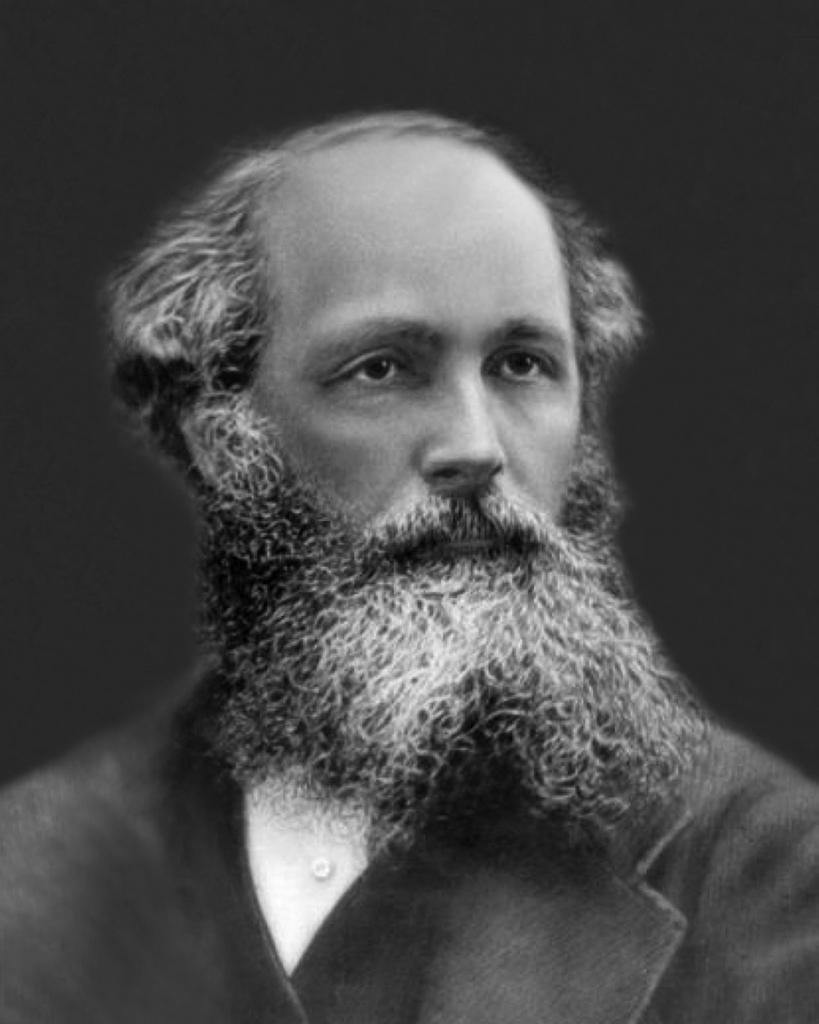
\includegraphics[width=0.4\textwidth]{figures/James-Clerk-Maxwell.jpg}
  %}{A picture of the Scottish physicist and mathematician James Clerk Maxwell from Wikimedia commons.}
    \caption{A picture of the Scottish physicist and mathematician James Clerk Maxwell from \href{https://upload.wikimedia.org/wikipedia/commons/b/b0/James-Clerk-Maxwell-1831-1879.jpg}{Wikimedia commons}.}
\end{figure}

If this confuses you then you are not alone. In the 1800's the Scottish Physicist James Clerk Maxwell had given a mathematical description of electricity and magnetism that unified them into the theory of \textbf{electromagnetism}. A consequence of this theory is that there are waves in the electromagnetic field, with light being an example of an electromagnetic wave. The theory also tells us that light always travels at the same speed, known as the speed of light $c=3\times 10^{8}\text{m/s}$.\\

Usually when we have waves they are travelling in a given medium. For example, water waves require water to move through, while sound waves are really pressure waves in the air or another substance.  This meant that many physicists expected there to be a medium, referred to as the \textbf{luminiferous aether} that light was a wave in. However, a range of experiments carried out by the American Physicists Michelson and Morley, showed that there was no such medium. This meant that an alternative explanation was needed for why light always travelled at the same speed regardless of how fast the object emitting light is travelling.\\

\begin{figure}[ht]
    \centering
    %\pdftooltip{
    \ThisAltText{ A picture of Albert Einstein from Wikimedia commons.}
    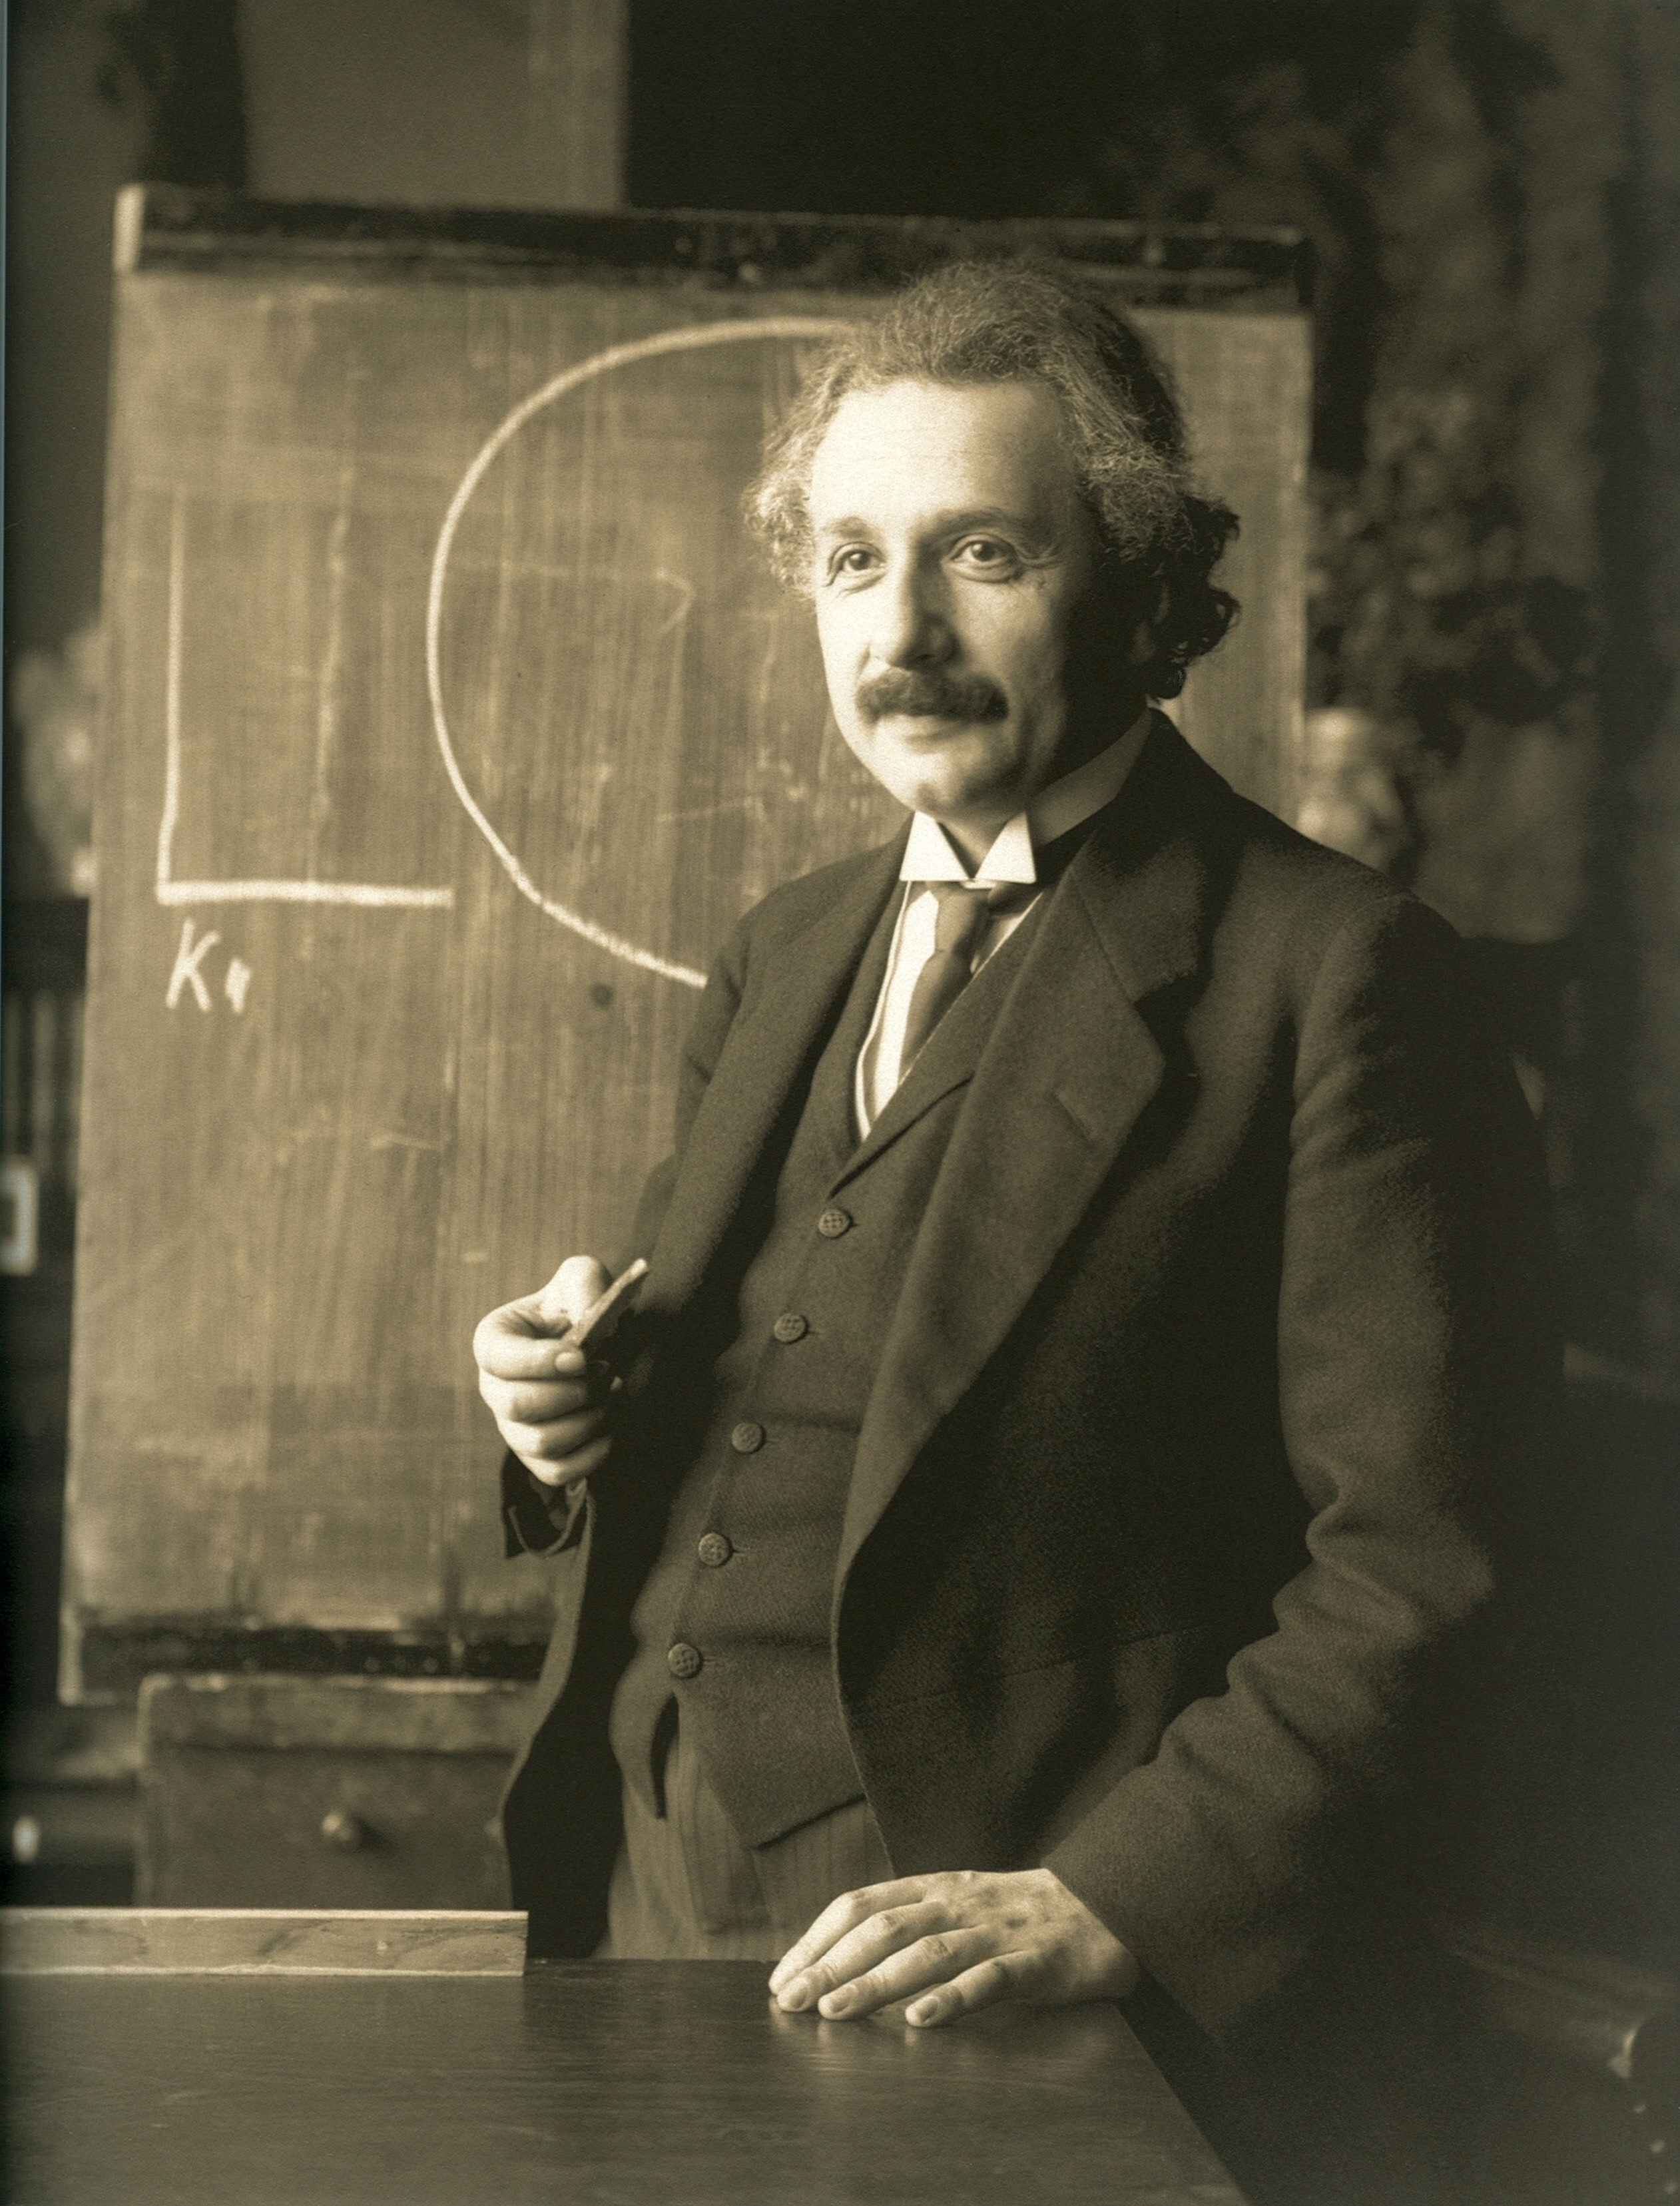
\includegraphics[width=0.4\textwidth]{figures/Einstein_1921_by_F_Schmutzer_-_restoration.jpg}
    %}{A picture of the German Physicist Albert Einstein from Wikimedia commons.}
    \caption{A picture of the German physicist Albert Einstein from \href{https://upload.wikimedia.org/wikipedia/commons/3/3e/Einstein_1921_by_F_Schmutzer_-_restoration.jpg}{Wikimedia commons}.}
\end{figure}

The eventual explanation was Einstein's theories of relativity, both \textbf{special relativity} and \textbf{general relatvity}.  Special relativity is based on two postulates:
\begin{itemize}
\setlength{\itemsep}{-5pt}
    \item[First:] The laws of physics are the same in all inertial frames.
    \item[Second:] The speed of light in vacuum is the same in all inertial frames.
\end{itemize}  

The second postulate implies that nothing can travel faster than the speed of light in vacuum $c=3\times 10^{8}\text{m/s}$. An important phrase in the postulates is \textbf{inertial frame}, this means that whoever is making the measurements is not accelerating. The word frame in the above postulates may seem confusing but it is just away of referring to a set of coordinate axes that move with an observer. So far in the module we have treated the coordinates $x,y,z$ and the time $t$ as absolute quantities that everyone performing measurements agrees on. However, a consequence of relativity is that this is not true, and the measurements that you make depend on how fast you are travelling.\\

This means that the Newtonian mechanics we studied throughout this module breaks down at high speeds. Do not despair about this, it does not mean that you should just bin everything that you have learnt so far. Everything that you have learnt is still valid, as long as you are not interested in very fast or massive objects. We will make this more precise shortly.\\

Consider a person moving with speed $v$ in the $x$ direction. \cref{fig: moving frames} shows the difference between the coordinates that our moving observer would use, and the coordinates that a stationary observer would use. By inspection of the figure we see that since the observer is only moving in the $x$-direction anything measured in $y$ and $z$ remains the same, this means that $y'=y,\,z'=z$.\\

\begin{figure}[ht]
    \centering
    \ThisAltText{ The Galilean relativity relationship between moving frames.}
    %\pdftooltip{
    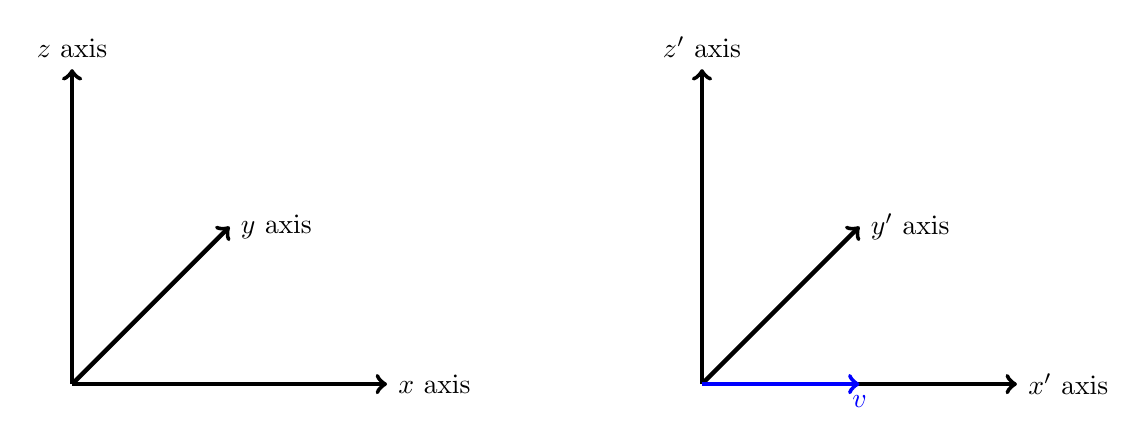
\begin{tikzpicture}
\draw[black, ultra thick,->] (0,0) --(4,0) node[anchor=west]{$x$ axis};
\draw[black, ultra thick,->] (0,0) --(2,2) node[anchor=west]{$y$ axis};
\draw[black, ultra thick,->] (0,0) --(0,4) node[anchor=south]{$z$ axis};
\draw[black, ultra thick,->] (8,0) --(12,0) node[anchor=west]{$x'$ axis};
\draw[black, ultra thick,->] (8,0) --(10,2) node[anchor=west]{$y'$ axis};
\draw[black, ultra thick,->] (8,0) --(8,4) node[anchor=south]{$z'$ axis};
\draw[blue, ultra thick, ->] (8,0) --(10,0) node[anchor=north]{$v$};
\end{tikzpicture}
%}{Comparison of a fixed frame with a frame moving at speed $v$ in the $x$-direction.}
    \caption{Comparison of a fixed frame with a frame moving at speed $v$ in the $x$-direction.}
    \label{fig: moving frames}
\end{figure} 

At slow speeds this is actually known as \textbf{Galilean relativity}, and we have that $x'=x-vt$. That is to convert from what is measured by the stationary observer to the moving observer we have to take account of how far the moving observer has travelled by the time they make the measurement. This sort of relativity does not pose any problems for what we have learnt in this module, the novelty comes if the observer is moving close to the speed of light. Then the relationship between $x$ and $x'$ is given by a different formula known as a \text{Lorentz transform}:
\begin{equation}
x'=\frac{x-vt}{\sqrt{1-\frac{v^{2}}{c^{2}}}}.
\label{eq: length contraction}
\end{equation}
More surprisingly, if the moving observer is carrying a clock, this will measure time at a different rate than a clock held by a stationary observer. This is something new and does not happen for Galilean relativity. If the clock held by a stationary observer shows a time $t$, then if they look at the clock held by the moving observer it will show a time
\begin{equation}
t'=\frac{t-\frac{v}{c^{2}}x}{\sqrt{1-\frac{v^{2}}{c^{2}}}}.
\label{eq: time dilation}
\end{equation}

The new part of these expressions is so important that it is called the \textbf{Lorentz factor}, or sometimes the gamma factor, and is given the symbol
\begin{equation}
\upgamma=\frac{1}{\sqrt{1-\frac{v^{2}}{c^{2}}}},
\end{equation}
some books will also call the ratio of the speed $v$ to the speed of light $\upbeta=v/c$.\\

An immediate consequence of these expressions is that a stationary observer will see the moving observer shrink\footnote{This is known as \textbf{length contraction}}, in the direction they are moving in, and will see the moving clock speeding up\footnote{This is known as \textbf{time dilation}}. The second phenomena is usually phrased from the point of view of the moving observer who will see the stationary observers clock moving more slowly than their own.\\

With length contraction, we can phrase it in a different way by. The length is the difference between two positions $x_{1}'$ and $x_{2}'$, we call the length measured in the moving frame $L_{0}=x_{2}'-x_{1}'$ and the length measured in the stationary frame $L$.
\begin{align*}
L_{0}&=x_{2}'-x_{1}'\\
	&=\frac{x_{2}-vt}{\sqrt{1-\frac{v^{2}}{c^{2}}}}-\frac{x_{1}-vt}{\sqrt{1-\frac{v^{2}}{c^{2}}}}\\
	&=\frac{x_{2}-x_{1}}{\sqrt{1-\frac{v^{2}}{c^{2}}}}\\
	&=\upgamma L.
\end{align*}

\paragraph{Example 9.1:} The Voyager spacecraft has a length of $4\text{m}$ and is moving at $12 260\text{m/s}$. How long does it appear to an observer on Earth?\\

We are given the length in the moving frame $L_{0}=4\text{m}$ so we just need to compute 
\begin{equation*}
\upgamma=\frac{1}{\sqrt{1-\frac{v^{2}}{c^{2}}}}=\frac{1}{\sqrt{1-\frac{(17260)^{2}}{(3\times10^{8})^{2}}}}=\frac{1}{0.9999999834496}=1.000000001655042.
\end{equation*}
We then know that $L_{0}=L\upgamma$ or $L=L_{0}/\upgamma$ so
\begin{equation*}
L=\frac{L_{0}}{\upgamma}=4\times0.9999999834496=3.99999999337981\text{m}.
\end{equation*}

This is a very small difference, and shows you just how fast an object has to be travelling for there to be an observable difference in the length. To find when the change in length is considerable we can compute the gamma factor for $v=c/2$,
\begin{equation*}
\upgamma=\frac{1}{\sqrt{1-\frac{1}{4}}}=\frac{2}{\sqrt{3}}=1.1547,
\end{equation*}
and for $v=9c/10$,
\begin{equation*}
\upgamma=\frac{1}{\sqrt{1-\frac{81}{100}}}=\frac{10}{\sqrt{19}}=2.29.
\end{equation*}
What do these mean for the observed length of voyager from Earth:
\begin{align*}
\text{for } v=c/2 \quad L&=\frac{L_{0}}{\upgamma}=\frac{4}{1.1547}=3.46\text{m},\\
\text{for } v=9c/10 \quad L&=\frac{L_{0}}{\upgamma}=\frac{4}{2.29}=1.74\text{m},
\end{align*}
so at both of these speeds we see a much more significant change in the length.\\

So far we have just been sketching out what happens when objects are moving very quickly. Another consequence of special relativity is the relationship of mass and energy through,
\begin{equation}
E=mc^{2}.
\end{equation}
This is another of Einstein's famous results, and says that every object has an intrinsic energy associated with its mass. This is a very important relationship if you are interested in nuclear energy as it is this intrinsic mass energy which is accessed via fission and fusion. \\

There is also general relativity which is Einstein's theory of gravitation, but this is a much more complicated story and we will not say anything about it here.

\section{Quantum Quandaries}
Now we turn from the very fast to the very small.  For an introduction to the wonderful world of quantum physics I recommend the 43rd and 44th videos from the crash course physics playlist available \href{https://www.youtube.com/playlist?list=PL8dPuuaLjXtN0ge7yDk_UA0ldZJdhwkoV}{here}.  The book \textbf{Quantum Physics: A Beginner's Guide } by Rae, \citep{rae2005quantum}, is available in the library and is a good jumping off point if you want to learn more about the counter intuitive world of quantum physics.\\

Quantum physics deals with the very smallest objects. These are fundamental particles like the electron, which we met as the charge carrier responsible for electric current. In most of this module we have thought in terms of balls rolling down slopes, juggling balls moving along a parabola, springs pendulums oscillating backwards and forwards. You may also have seen artists impressions of atoms where they are represented as being mini solar systems with the electrons orbiting around a central positively charged nucleus.  However, this is not really what is going on.\\

At the smallest scale, particles are waves and waves are particles!\\

You are probably asking ``what does this mean?'' The answer is that what you observe when you look at something depends on how you look at it. \\

The most famous example of this is what is known as the double slit experiment. If we imagine having two screens set up, one with two slits cut in it so that can pass through the holes in the first screen and then hit the second screen. This is shown for classical particles and waves in \cref{fig: double slit particle,fig: double slit waves} respectively. For classical particles they either pass through one slit or the other and will strike the second screen in line with the slits. This would result in the pattern shown in \cref{fig: double slit particle}.\\

\begin{figure}[ht]
    \centering
    \ThisAltText{ A picture of the double slit experiment for particles taken from Wikimedia commons.}
   % \pdftooltip{
   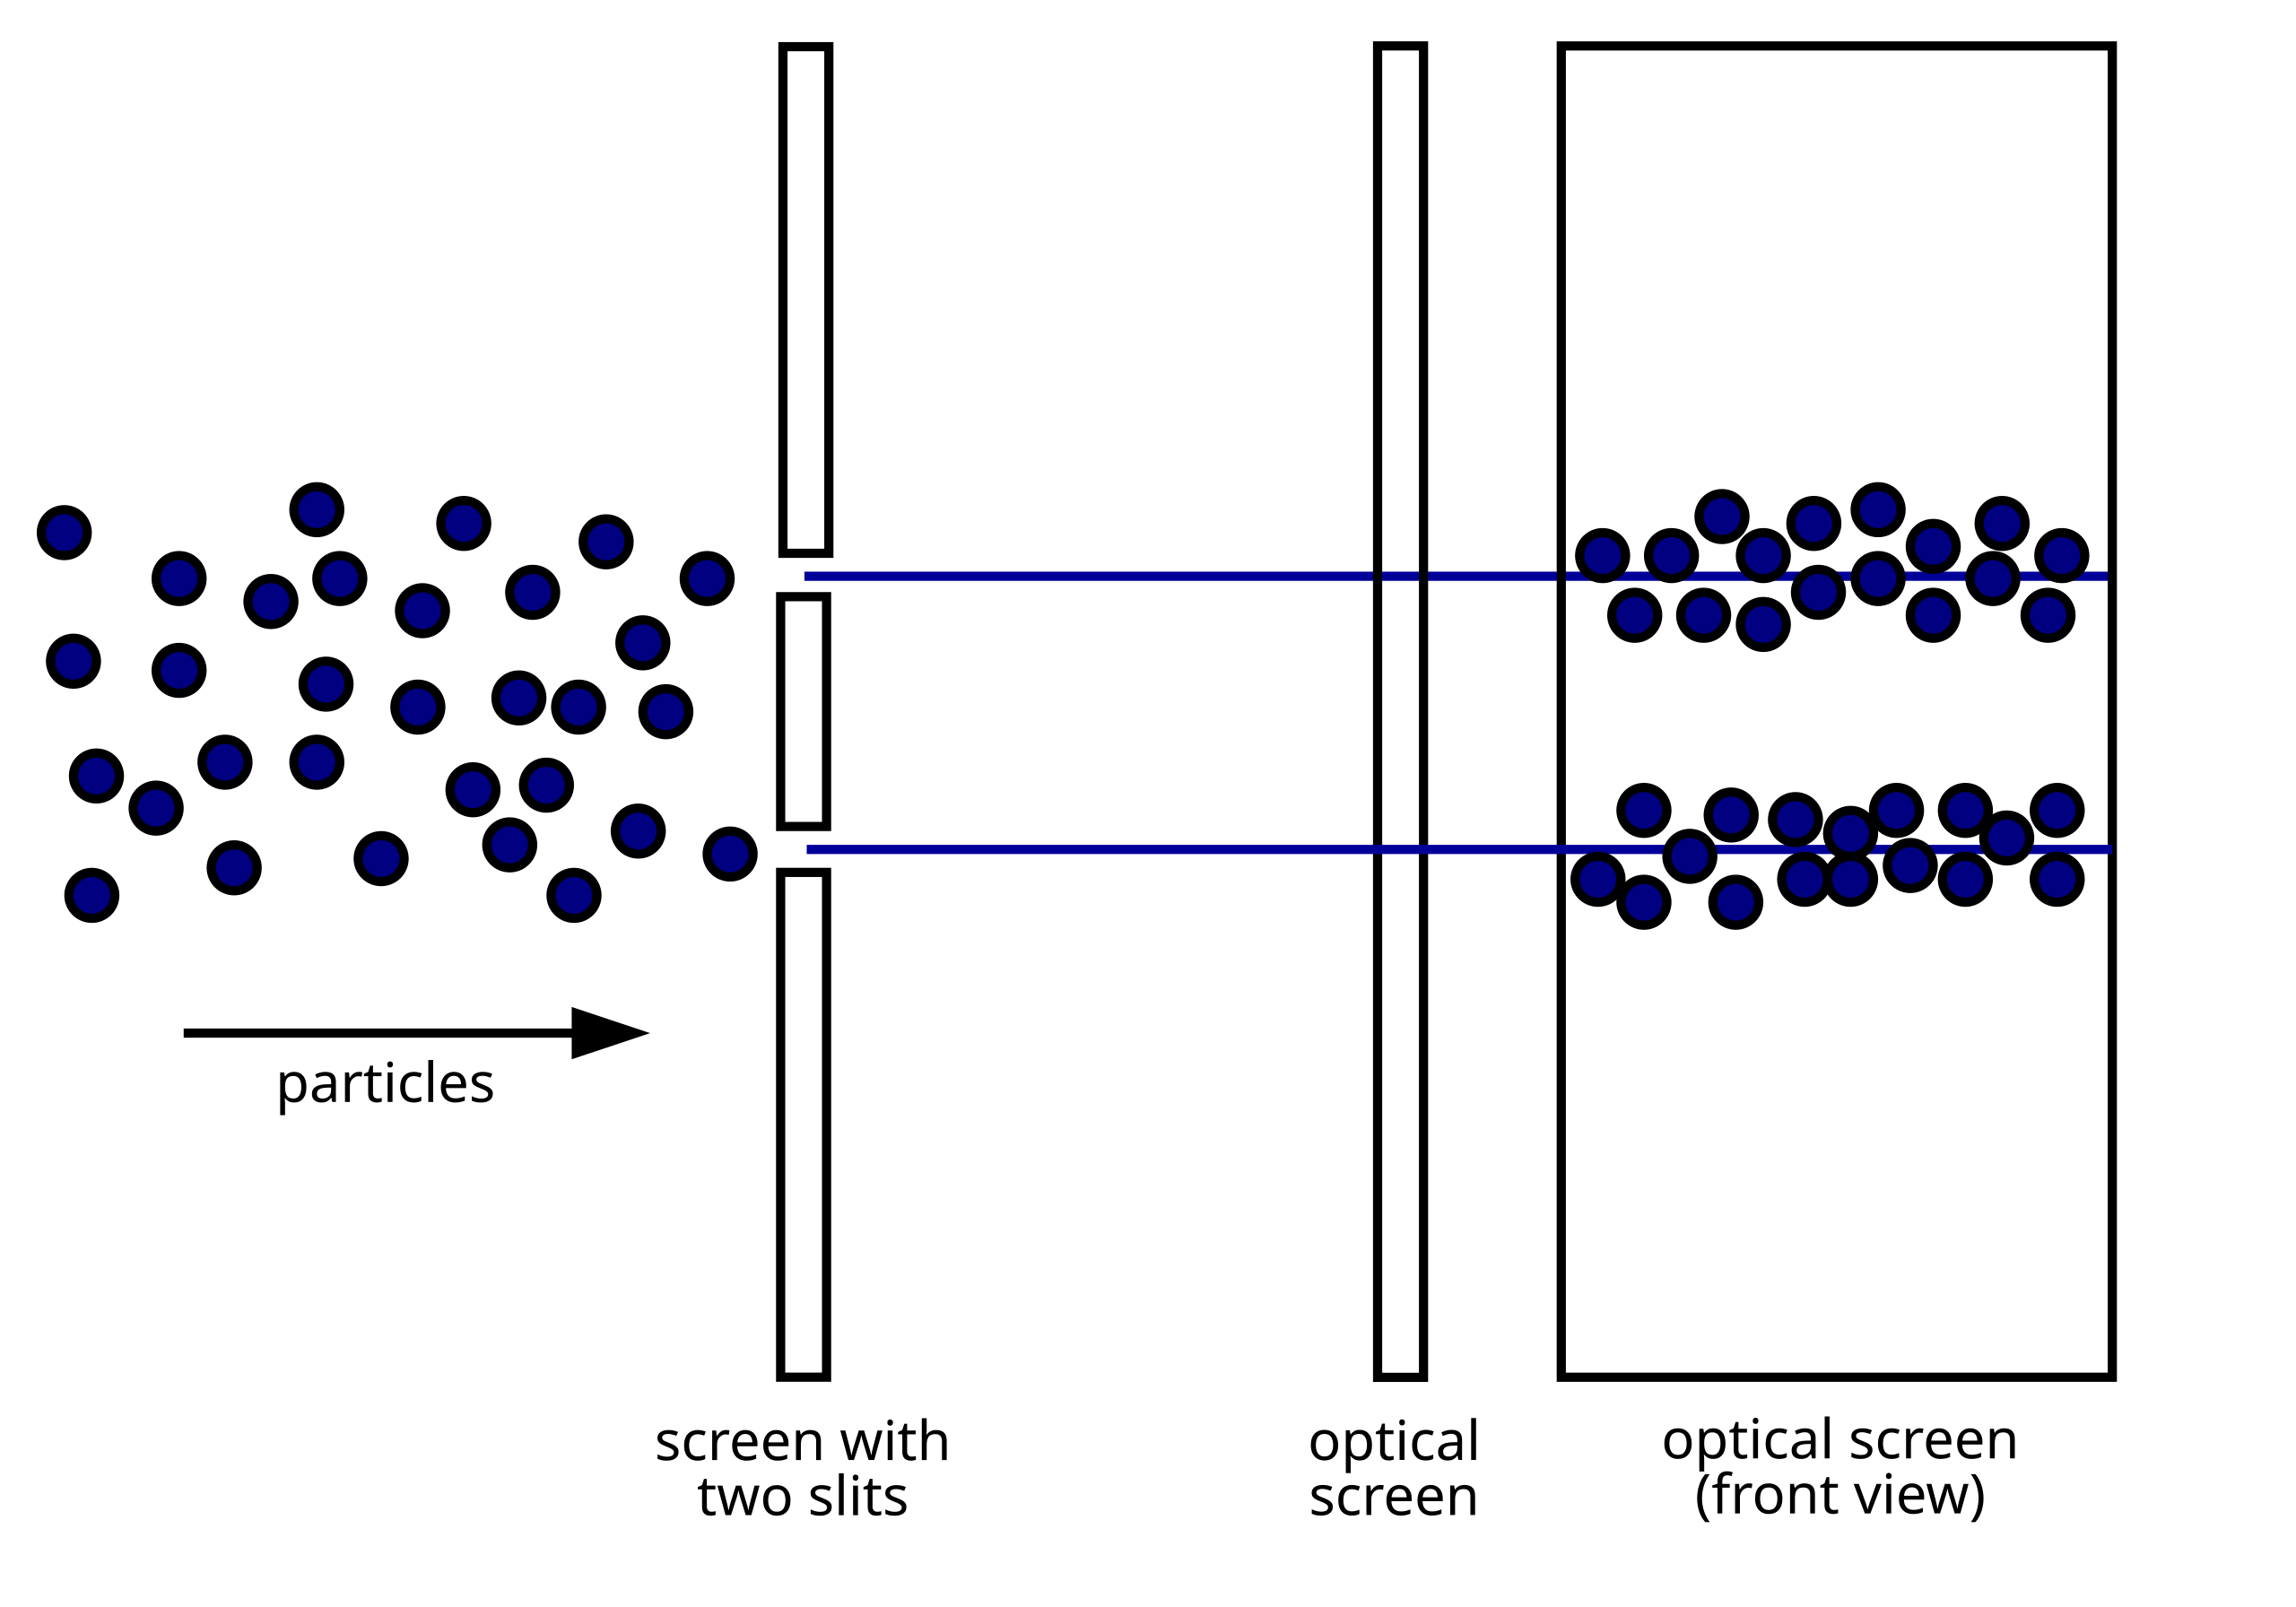
\includegraphics[width=0.5\textwidth]{figures/Two-Slit_Experiment_Particles.png}
   %}{A picture of the double slit experiment for particles from Wikimedia commons.}
    \caption{A picture of the double slit experiment for particles from \href{https://commons.wikimedia.org/wiki/File:Two-Slit_Experiment_Particles.svg}{Wikimedia commons}.}
    \label{fig: double slit particle}
\end{figure}

When a wave passes through a slit it \textbf{diffracts}\footnote{This means that it bends as it passes through the aperture. Diffraction is one of the hallmark behaviour of waves.}. When there are two slits the wave passes through both and diffracts so we have two sets of wavefronts one emerging from each of the slits. These wavefronts then \textbf{interfere}\footnote{Interference is another hallmark behaviour of waves. It means that when two waves overlap they add together so if a peak lies on top of a peak this leads to a wave with an even bigger peak, if a trough lies on top of a trough it leads to an even deeper trough, both called constructive interference. While if a peak lies on top of a trough they cancel out, called destructive interference.. } with each other, and we see an interference pattern on the second screen. This means that there is an intensity peak in the middle of the screen, with a sequence of peaks of decreasing brightness spread out on the screen. This is shown in \cref{fig: double slit waves}.\\

\begin{figure}[ht]
    \centering
    \ThisAltText{ A picture of the double slit experiment for waves taken from Wikimedia commons.}
    %\pdftooltip{
    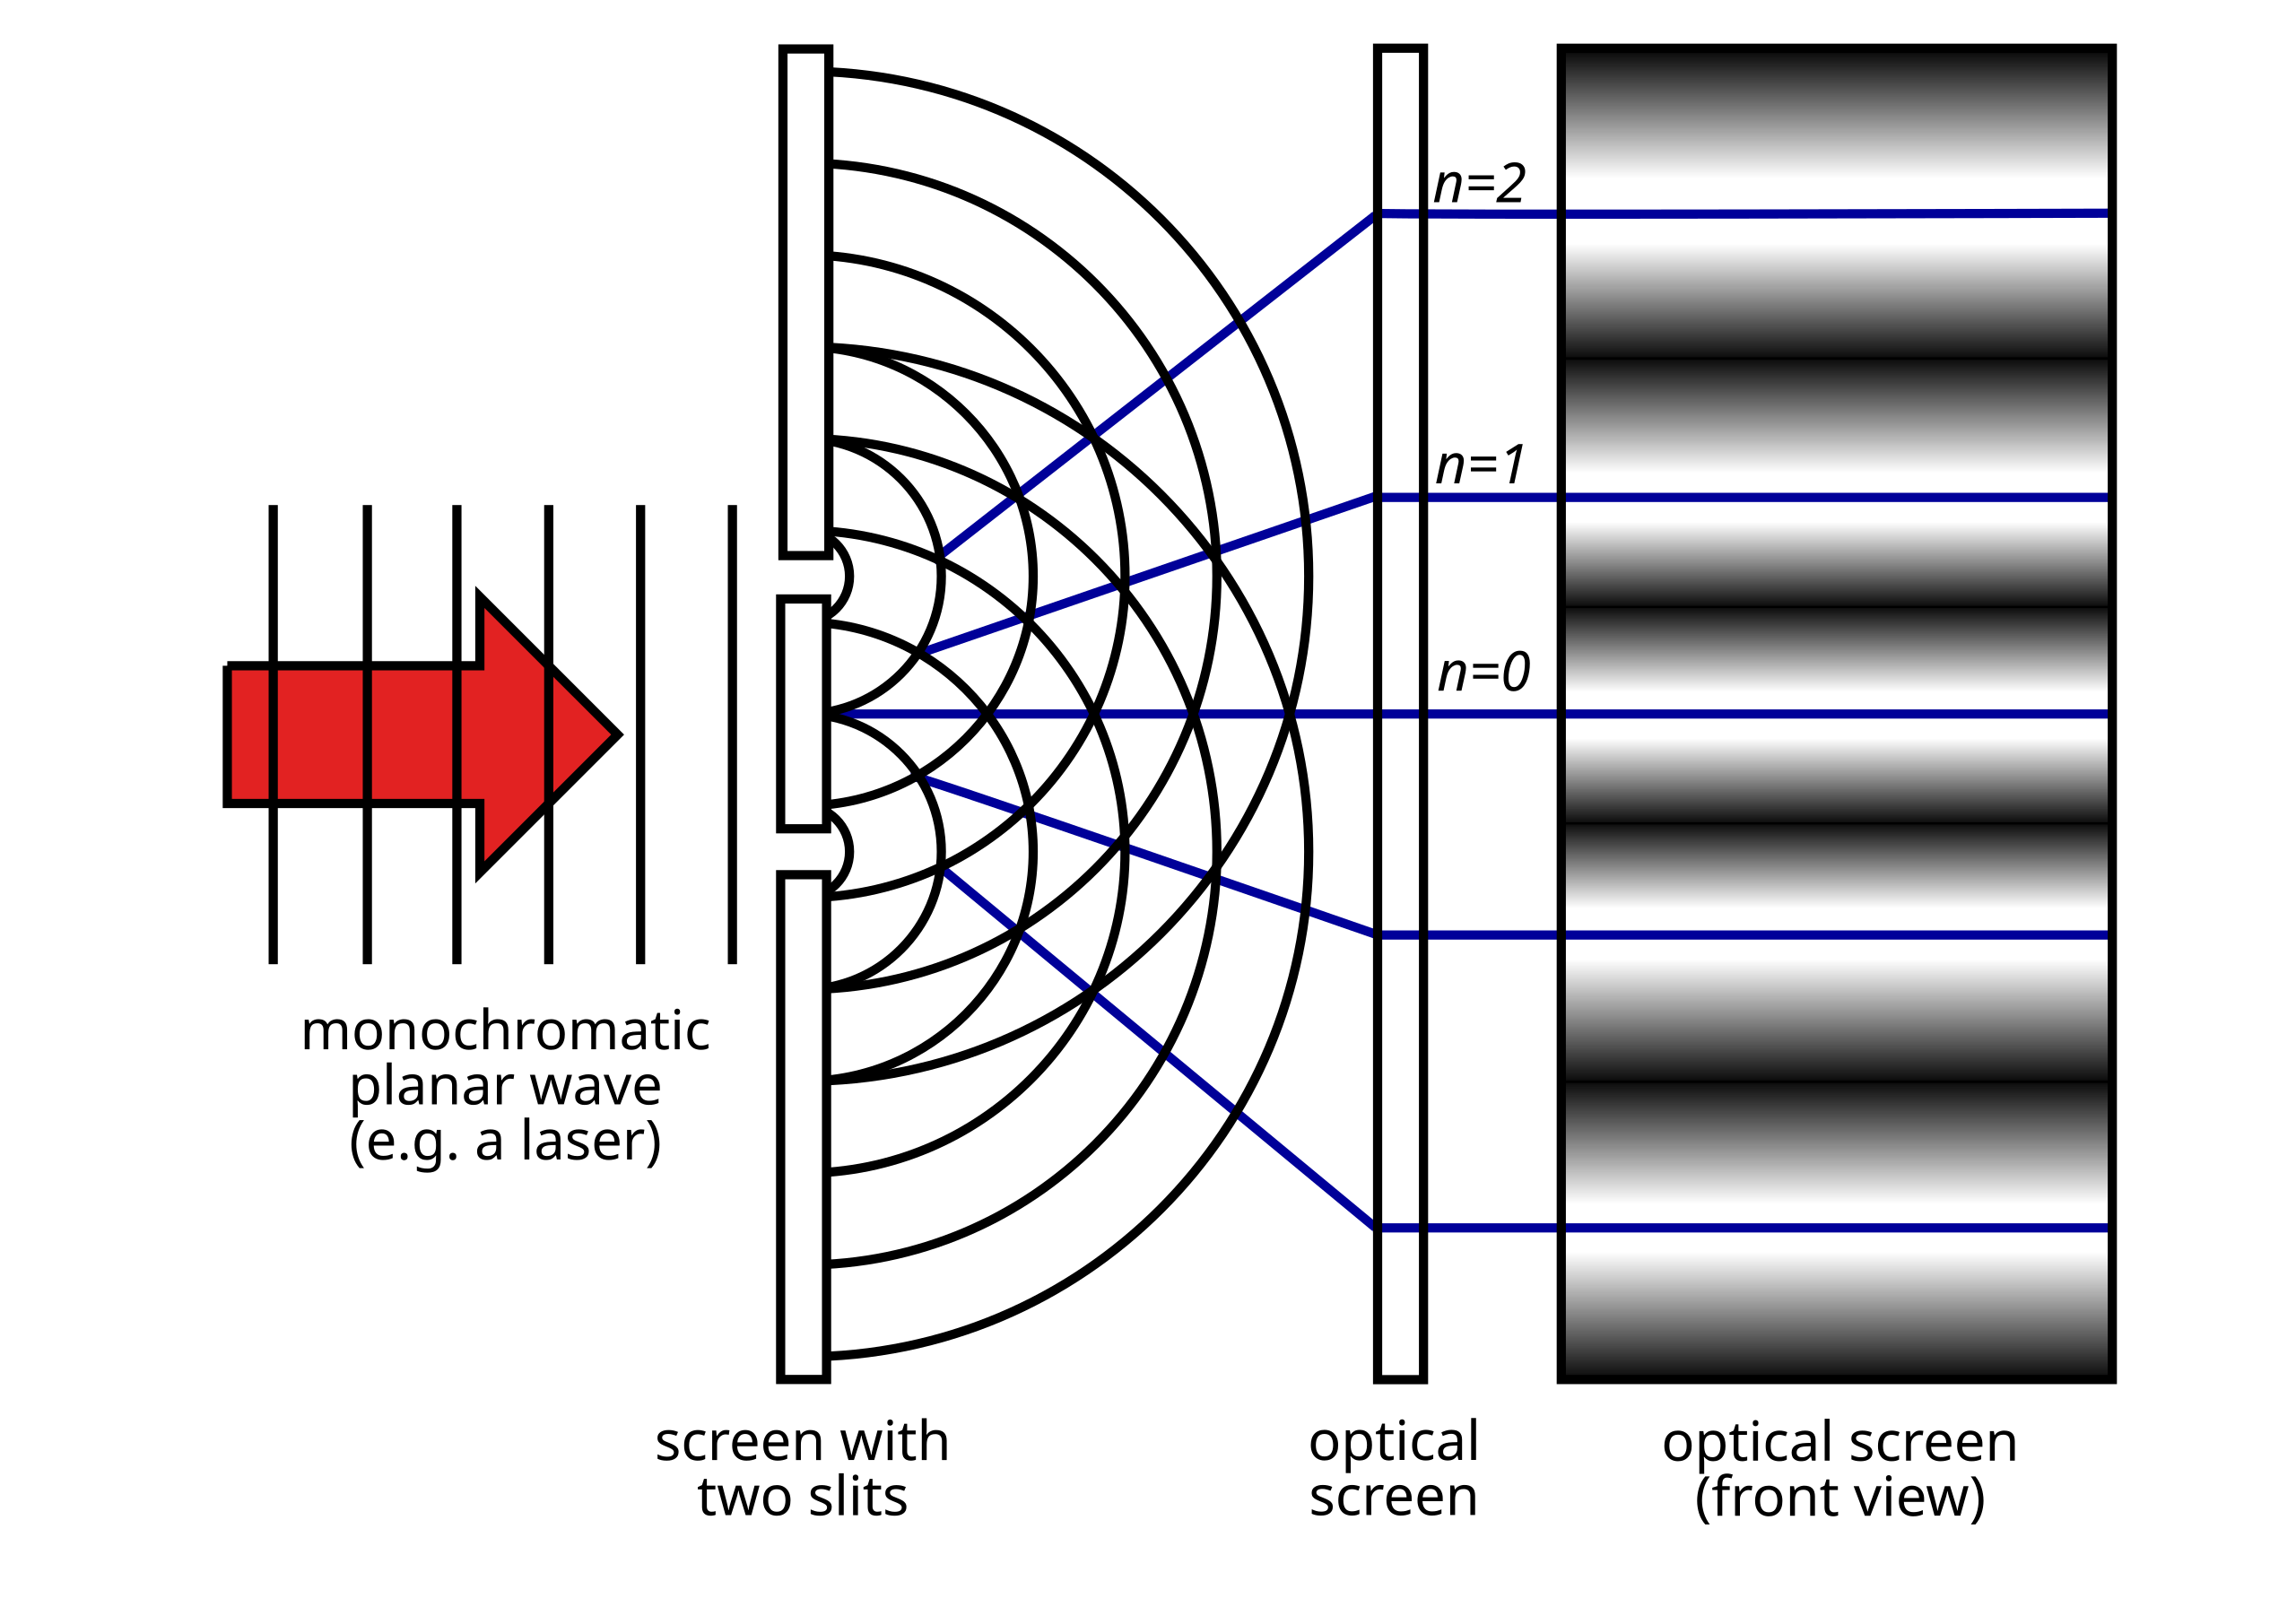
\includegraphics[width=0.5\textwidth]{figures/Two-Slit_Experiment_Light.png}
    %}{A picture of the double slit experiment for waves from Wikimedia commons.}
    \caption{A picture of the double slit experiment for waves from \href{https://commons.wikimedia.org/wiki/File:Two-Slit_Experiment_Light.svg}{Wikimedia commons}.}
    \label{fig: double slit waves}
\end{figure}

The double slit experiment was first performed by Thomas Young in 1801 and was taken as a demonstration that light behaved like a wave, as Young observed the wave-like interference pattern. However, at the turn of the twentieth century both Max Planck and Albert Einstein gave theoretical evidence that light should be treated as a particle in certain circumstances. Planck did this to explain \textbf{black-body radiation}, the radiation emitted by a body in thermal equilibrium with its environment. While Einstein presented a solution to the \textbf{photoelectric effect}, the emission of electrons from a material when light with a specific wavelength is shone on the material. Both of these explanations rely on thinking of light as being made up of \textbf{quanta}, or lumps, of energy known as \textbf{photons}. This is the first evidence of what is known as \textbf{wave-particle duality}, the fact that some objects can behave like a wave or a particle depending how you look at them. \\

In the 1920's the French Physicists Louis de Broglie took this a step further and proposed that objects like electrons and protons that were thought of as being particles, could behave like waves in certain circumstances. This was then tested by carrying out a double slit experiment for electrons, see \cref{fig: double slit electrons} for a schematic of this.  It turns out that even if you slow this down so much that only one electron at a time is being emitted, you still see an interference pattern so somehow the electron is interfering with itself.\\

It is natural to ask if we can just watch one of the slits and see does the electron pass through or not. If we do this then we will either see an electron pass through or not, but now on the second screen we observe the particle like picture from \cref{fig: double slit particle}. The surprising results is that if you try to observe a particle like property of an electron, or any other sub atomic particle, you get a particle like answer, while if you try to observe a wave like property you get a wave like answer.\\

\begin{figure}[ht]
    \centering
    %\pdftooltip{
    \ThisAltText{ A picture of the double slit experiment for quantum objects taken from Wikimedia commons.}
    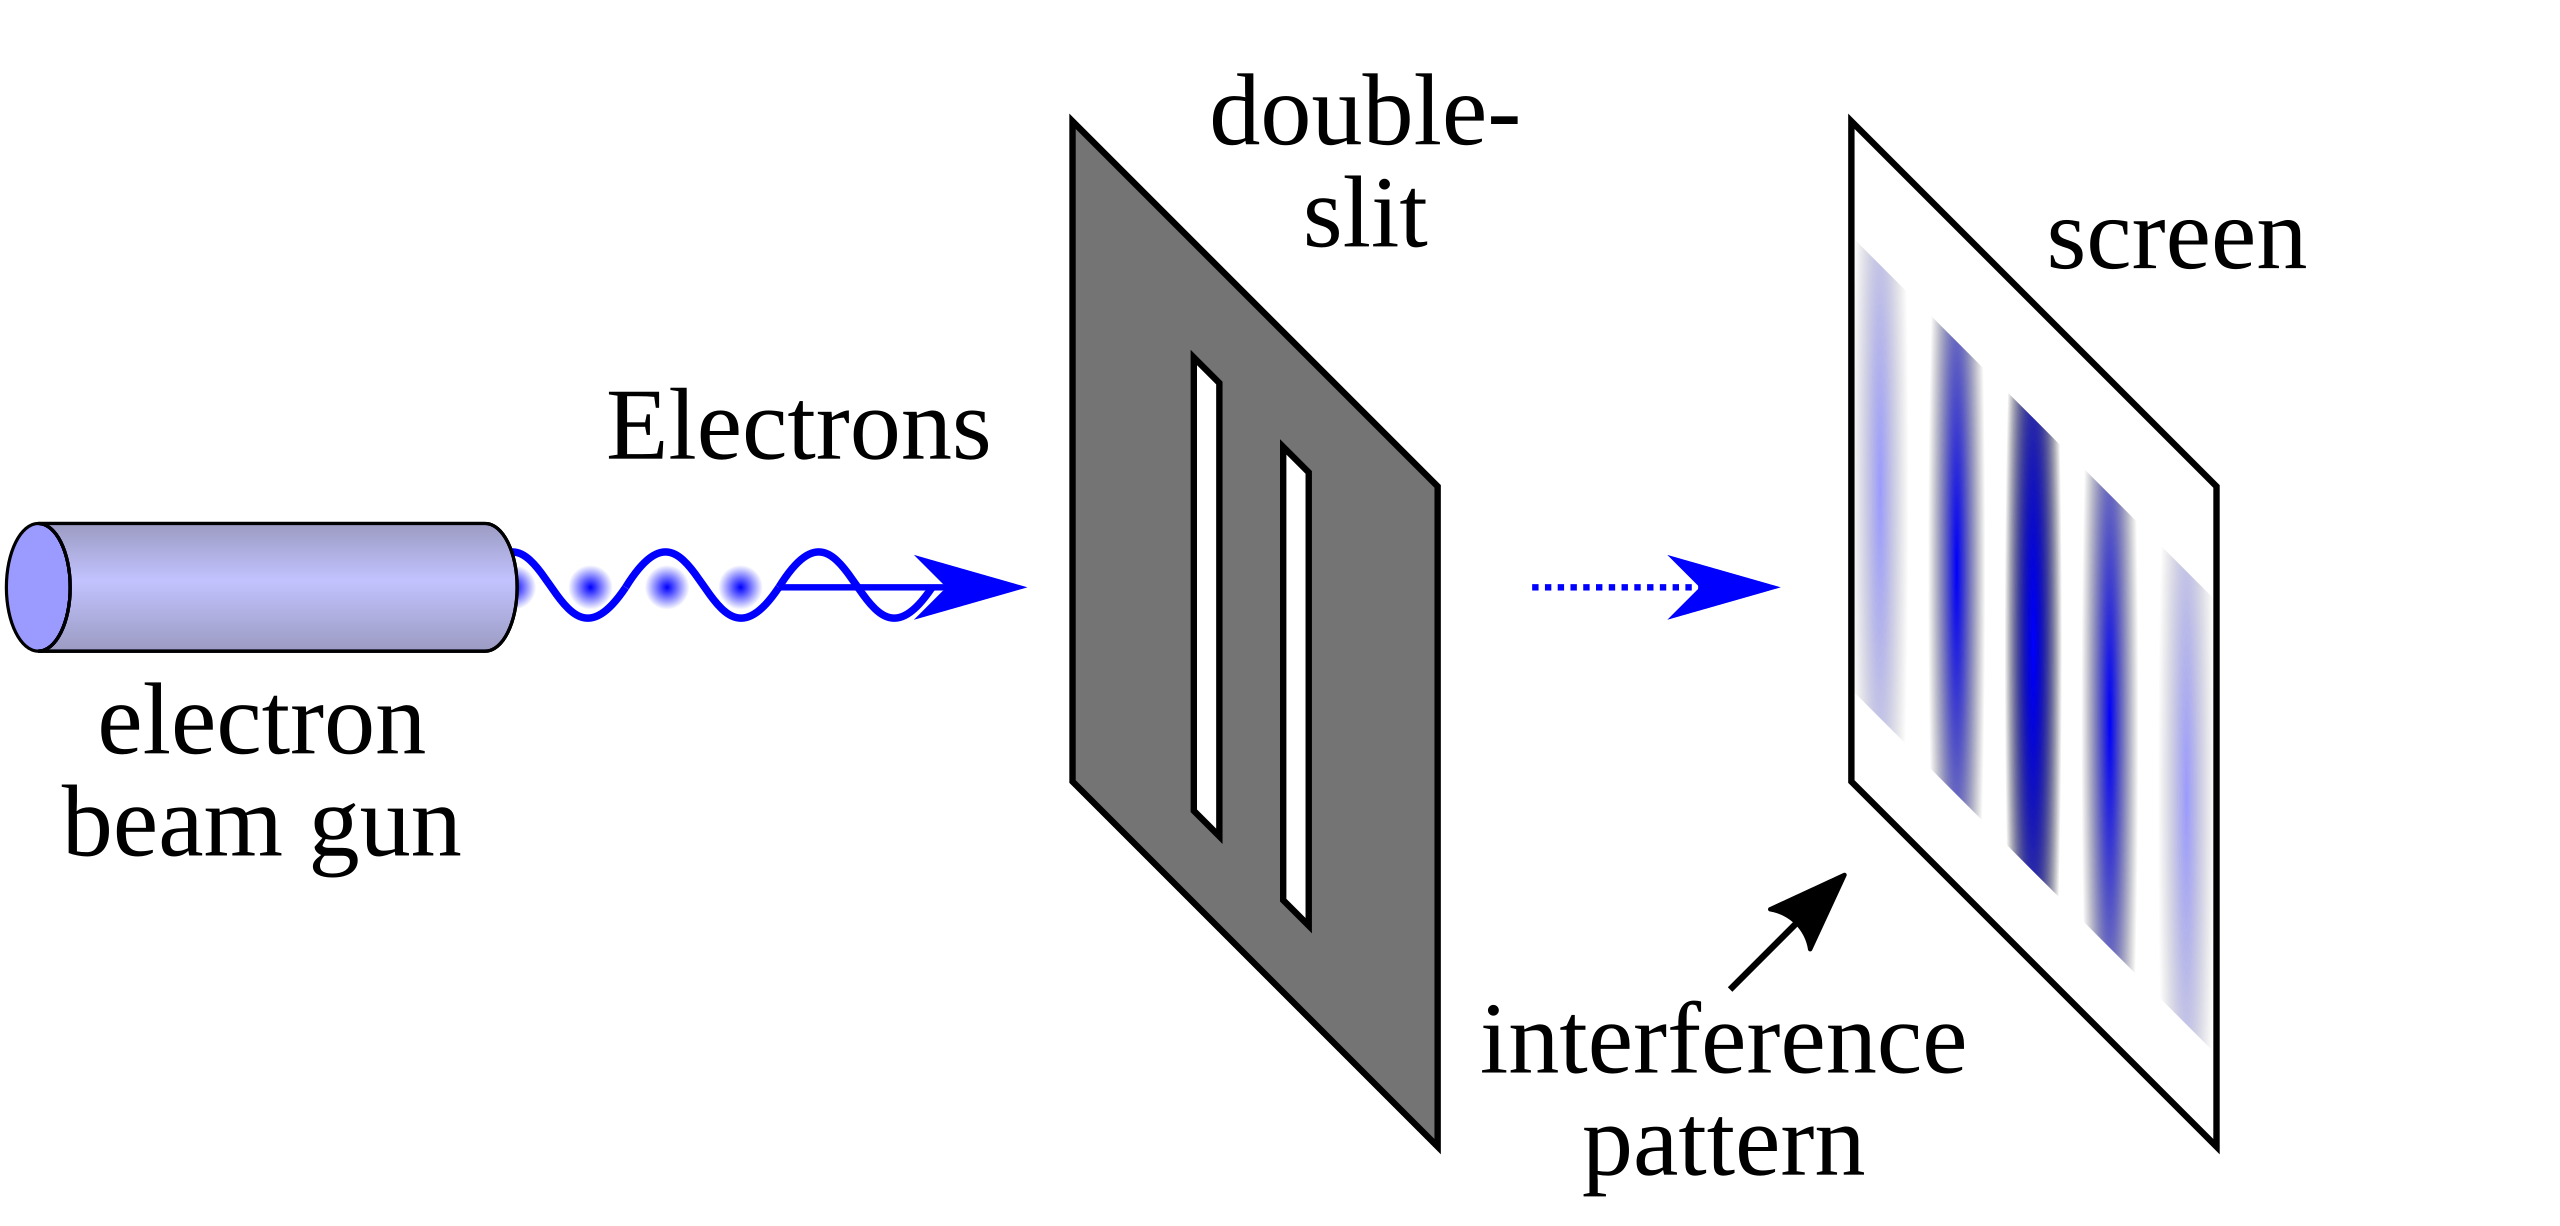
\includegraphics[width=0.5\textwidth]{figures/double_slit_electrons.png}
    %}{A picture of the double slit experiment for electrons from Wikimedia commons.}
    \caption{A picture of the double slit experiment for electrons from \href{https://commons.wikimedia.org/wiki/File:Double-slit.svg}{Wikimedia commons}.}
    \label{fig: double slit electrons}
\end{figure}

If this sounds completely crazy to you then you are not alone. It is an incredibly counter intuitive observation, in the everyday world a football does not swap between being a solid ball and a wave depending on how I observe it. However on the quantum scale this really does happen. Discoveries like this lead the physicist Richard Feynman to say ``Nobody understands quantum mechanics'', and leads on to a school of thought called ``shut up and calculate''. This point of view is essentially that you should forget about trying to draw pictures of what is going on  and trying to describe complete trajectories. Instead focus on what you can observe, and let the mathematics guide you. 
